\chapter{Case study: LoRa}
\label{chap:case-staudyLoRa}

This chapter presents the case study used as reference scenario during the evolution of the DingNet simulator, and to evaluate the limits of communication from applications to LoRa motes. 
A demo from this case study was showed during the Day of Science in Flanders to present the LoRaWAN technology receiving a lot of attention.

\section{Description case study}

We want to realize a system able to provide to the user the healthiest route to reach a destination. 
The route generation will be based on air quality level of the areas to across to reach the destination. 
The user, in order to obtain the route, has to require it to the application deployed in a remote server.
The system use the data received from the sensor network to create a city map of quality air.
Then, the application has to define the route to a destination that optimize the trade-off between air quality and length of the route.
The system should be able to recompute the best route if the environment condition change, and communicate it to the user.
The sensor network can be composed by two types of sensors:
\begin{itemize}
    \item \textbf{Fixed}: positioned along the roads and at intersections
    \item \textbf{Mobile}: placed on public transport or bicycles
\end{itemize}
All the sensors have to be deployed in a LoRaWan network, similarly also the user device, that will interact with the application to require the route, has to use the LoRa technology.

\section{Design of the system}
\autoref{fig:caseStudyA} shows the high level architecture of the system, and introduce the main entities. 
The main entities are the sensor devices, the user devices, and the routing application.
As requirement both the sensor devices and the user devices have to be displaced inside the LoRaWAN network and use the LoRa technology to communicate with the routing application.
Using the DingNet simulator to simulate the LoRaWAN network:
\begin{itemize}
    \item the routing application is mapped in a generic application presents in the application server that communicates with the LoRaWAN network via MQTT
    \item the sensor devices, that have to send only packet with the sensed value, can be mapped in the \textit{Mote} simulator entity
    \item the user devices are special devices, because they do not send only packets with the sensed value, but have also to require the route for a destination and be able to manage the received packets with the route. Actually there isn't present a simulator entity with this specific abilities, so it will be necessary to define it.
\end{itemize}
% 
\begin{figure}[h]
    \centering
    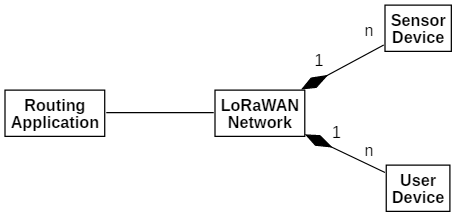
\includegraphics{figures/CaseStudyA_HLarch.png}
    \caption{High level architecture of the system}
    \label{fig:caseStudyA}
\end{figure}
% 
\subsection*{Interaction between application and devices}
If on one hand the transmissions from the devices (both sensor and user) to the application are in compliance with the maximum packet's length defined by the LoRaWAN standard (1 byte for packets with the sensed value, and 16 bytes for the packet to require the route), on the other hand it is impossible to send the packet from application to the user device with the entire route, so the only way to send it is to split it in more packets.
In order to send the entire route to the user device are possible two approaches: 
\begin{enumerate}
    \item define a specific interaction protocol to send all the packets with the entire route to the user device immediately after its computation
    \item send a packet with a part of the route only when the user have finish the previous part of the route.
\end{enumerate}
Considering also the requirement to recompute the route if the environment condition change it was chosen the second option, enabling to recompute the route before send its next part.

\subsection*{Design of the user device}
% UserMote - consume packet
The user device has to perform three activity: require the route, send update of its position, and manage the incoming packets.
If on one hand the last two activity can be performed also from a \textit{Mote}, on the other hand it cannot require the route.
For this reason in \autoref{fig:userMote} is introduced a new entity simulator, the \textit{UserMote} that extends the \textit{Mote} adding the logic to require the route when needed sending a packet with starting and destination positions.
Then to manage incoming packets are chosen \textit{MaintainLastPacket} as strategy to store packets until that they are consumed, and \textit{ReplacePath} as only strategy to consume packets. It consume each packet updating the user route in accord with the packet content until the route is completed.
To perform the last activity, send updating of the user position, is necessary add the GPS sensor to the \textit{UserMote}, and send it when the user is closer to the destination of sub-route.
% 
\begin{figure}[h]
    \centering
    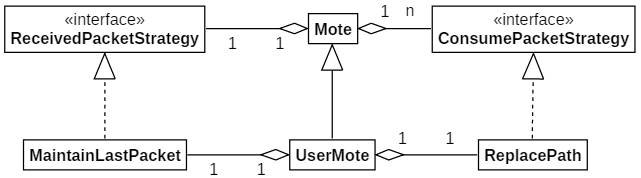
\includegraphics{figures/userMote.png}
    \caption{\textit{UserMote} model.}
    \label{fig:userMote}
\end{figure}
% 

\subsection*{Routing application}
% applicazione - comunicazione via MQTT
The application to found the best route implements an A-star algorithm on the graph of street of the city. 
The weight of the edges of the graph corresponds to the distance between the two points multiply for a factor that represent the air quality level in that street. 
The values sensed by the sensors are retrieved subscribing the topics where the LoRaWAN networks publish them, and the route is send to the user mote publishing the massage with sub-route in its receiving topic.
The application recompute the best route only when the user device communicate its new position and if some environment condition is changed from the previous computation.

% Demo + discussion limitazioni ed utilità del caso di studio????